\documentclass[a4paper,14pt]{extarticle}
\usepackage[utf8]{inputenc}
\usepackage[T1, T2A]{fontenc}
\usepackage[english, russian]{babel}
\usepackage{array}
\usepackage{ulem}
\usepackage{graphicx}
\usepackage{geometry}
\usepackage{amsmath, amssymb, amsthm, mathtools}
\usepackage{makecell}
\usepackage{booktabs}
\usepackage{listings}
\usepackage{xcolor}
\usepackage{upquote}
\lstset{extendedchars=true, inputencoding=utf8}
\usepackage{import}
\usepackage{subcaption}
\usepackage{float}
\usepackage{amsfonts}
\usepackage[hidelinks]{hyperref}
\usepackage{indentfirst}
\usepackage{tabularx}
\usepackage{bookmark}


\definecolor{codegreen}{rgb}{0,0.6,0}
\definecolor{codegray}{rgb}{0.5,0.5,0.5}
\definecolor{codepurple}{rgb}{0.58,0,0.82}
\definecolor{backcolour}{rgb}{0.95,0.95,0.92}

\lstdefinestyle{mystyle}{
    backgroundcolor=\color{backcolour},
    commentstyle=\color{codegreen},
    keywordstyle=\color{magenta},
    numberstyle=\tiny\color{codegray},
    stringstyle=\color{codepurple},
    basicstyle=\ttfamily\footnotesize,
    breakatwhitespace=false,
    breaklines=true,
    captionpos=b,
    keepspaces=true,
    numbers=left,
    numbersep=5pt,
    showspaces=false,
    showstringspaces=false,
    showtabs=false,
    tabsize=2
}

\lstset{
    style=mystyle,
    extendedchars=true,
    literate={а}{{\selectfont\char224}}1
    {б}{{\selectfont\char225}}1
    {в}{{\selectfont\char226}}1
    {г}{{\selectfont\char227}}1
    {д}{{\selectfont\char228}}1
    {е}{{\selectfont\char229}}1
    {ё}{{\"e}}1
    {ж}{{\selectfont\char230}}1
    {з}{{\selectfont\char231}}1
    {и}{{\selectfont\char232}}1
    {й}{{\selectfont\char233}}1
    {к}{{\selectfont\char234}}1
    {л}{{\selectfont\char235}}1
    {м}{{\selectfont\char236}}1
    {н}{{\selectfont\char237}}1
    {о}{{\selectfont\char238}}1
    {п}{{\selectfont\char239}}1
    {р}{{\selectfont\char240}}1
    {с}{{\selectfont\char241}}1
    {т}{{\selectfont\char242}}1
    {у}{{\selectfont\char243}}1
    {ф}{{\selectfont\char244}}1
    {х}{{\selectfont\char245}}1
    {ц}{{\selectfont\char246}}1
    {ч}{{\selectfont\char247}}1
    {ш}{{\selectfont\char248}}1
    {щ}{{\selectfont\char249}}1
    {ъ}{{\selectfont\char250}}1
    {ы}{{\selectfont\char251}}1
    {ь}{{\selectfont\char252}}1
    {э}{{\selectfont\char253}}1
    {ю}{{\selectfont\char254}}1
    {я}{{\selectfont\char255}}1
    {А}{{\selectfont\char192}}1
    {Б}{{\selectfont\char193}}1
    {В}{{\selectfont\char194}}1
    {Г}{{\selectfont\char195}}1
    {Д}{{\selectfont\char196}}1
    {Е}{{\selectfont\char197}}1
    {Ё}{{\"E}}1
    {Ж}{{\selectfont\char198}}1
    {З}{{\selectfont\char199}}1
    {И}{{\selectfont\char200}}1
    {Й}{{\selectfont\char201}}1
    {К}{{\selectfont\char202}}1
    {Л}{{\selectfont\char203}}1
    {М}{{\selectfont\char204}}1
    {Н}{{\selectfont\char205}}1
    {О}{{\selectfont\char206}}1
    {П}{{\selectfont\char207}}1
    {Р}{{\selectfont\char208}}1
    {С}{{\selectfont\char209}}1
    {Т}{{\selectfont\char210}}1
    {У}{{\selectfont\char211}}1
    {Ф}{{\selectfont\char212}}1
    {Х}{{\selectfont\char213}}1
    {Ц}{{\selectfont\char214}}1
    {Ч}{{\selectfont\char215}}1
    {Ш}{{\selectfont\char216}}1
    {Щ}{{\selectfont\char217}}1
    {Ъ}{{\selectfont\char218}}1
    {Ы}{{\selectfont\char219}}1
    {Ь}{{\selectfont\char220}}1
    {Э}{{\selectfont\char221}}1
    {Ю}{{\selectfont\char222}}1
    {Я}{{\selectfont\char223}}1
}

\geometry{
    a4paper,
    left=15mm,
    right=15mm,
    top=15mm,
    bottom=15mm
}

\begin{document}
% памятки
% \lstinputlisting[language=Python, caption={Построение графика исходной функции}]{code/func1.py}

\begin{titlepage}
    \begin{minipage}{0.45\textwidth}\raggedright
        \begin{center}
            \textbf{Университет ИТМО \\
            \vspace{0.1cm}
            Мегафакультет компьютерных технологий и управления \\
            \vspace{0.1cm}
            Факультет систем управления и робототехники
            }
        \end{center}
    \end{minipage}
    \hfill
    \noindent\begin{minipage}{0.4\textwidth}
    
\includegraphics[width=\linewidth]{imgs/logo-itmo.png}
    \end{minipage}

    \vspace{0.5cm}
    \hrule % Горизонтальная линия
    \vspace{0.5cm}

    % \begin{tabular}{|m{8cm}|m{8cm}|}
    \raggedright
     Работу выполнили: \uline{ Тарасов Степан, Мусаев Фуад, Пономарев Илья }\\
    \vspace{0.1cm}
    Преподаватель:  \uline{ Пашенко Артем Витальевич}\\
    \vspace{0.1cm}
    
    \vspace{0.5cm}
    \hrule % Горизонтальная линия
    \vspace{0.5cm}

    \vspace{3.5cm}
        
    \begin{center}
        \textbf{\Large ЛАБОРАТОРНАЯ РАБОТА №2}
    
        \vspace{0.7cm}
        \hrule % Горизонтальная линия
        \vspace{0.5cm}
    
        \textbf{\large{Преобразование Фурье}}
    
        \vspace{0.5cm}
        \hrule % Горизонтальная линия
        \vspace{1cm}
        
        \vfill
        Санкт-Петербург, 2026
    \end{center}
\end{titlepage}

\tableofcontents

\newpage
\section{Вещественное преобразование}

\subsection{Прямое преобразование Фурье}

Проведём аналитическое вычисление унитарного преобразования Фурье для заданных функций. Прямое преобразование осуществляется по следующей формуле, где симметричный нормировочный множитель $\frac{1}{\sqrt{2\pi}}$ также сохраняется и для обратного преобразования:
\begin{equation*}
    \hat{f}(\omega) = \frac{1}{\sqrt{2\pi}}\int\limits_{-\infty}^{\infty}f(t)e^{-i\omega t}dt
\end{equation*}

\textbf{Прямоугольная функция}
\begin{equation*}
f(t) = \begin{cases} 
a, & |t| \le b, \\ 
0, & |t| > b. 
\end{cases}
\end{equation*}

Выполним прямое интегрирование:
\begin{equation*}
\begin{split}
    \hat{f}(\omega) &= \frac{1}{\sqrt{2\pi}}\int\limits_{-b}^{b}ae^{-i\omega t}dt = -a\frac{1}{\sqrt{2\pi}}\frac{e^{-i\omega t}}{i\omega }\Bigg|_{-b}^{b} = a\frac{1}{\sqrt{2\pi}}\left(\frac{e^{i\omega b}}{i\omega } - \frac{e^{-i\omega b}}{i\omega}\right) =\\
    &= a\frac{1}{\sqrt{2\pi}}\frac{e^{i\omega b} - e^{-i\omega b}}{i\omega} = \frac{1}{\sqrt{2\pi}}\frac{2a \sin(\omega b)}{\omega }
\end{split}
\end{equation*}

\textbf{Треугольная функция}
\begin{equation*}
f(t) = \begin{cases} 
a - \frac{a}{b}|t|, & |t| \le b, \\ 
0, & |t| > b. 
\end{cases}
\end{equation*}

Поскольку аргумент находится под знаком модуля, данная функция является четной. Из свойств преобразования Фурье известно, что для четных функций мнимая часть интеграла (с синусом) обнуляется. Поэтому преобразование упрощается до интегрирования только с вещественной частью (косинусом):

\begin{equation*}
\begin{split}
    \hat{f}(\omega) &= \frac{1}{\sqrt{2\pi}}\int\limits_{0}^{b} 2\left(a-\frac{a}{b}t\right) \cos(\omega t)dt = \frac{1}{\sqrt{2\pi}}\left(2a \int_{0}^{b} \cos(\omega t) dt - \frac{2a}{b} \int_{0}^{b} t \cos(\omega t) dt\right) =\\
    &= \frac{1}{\sqrt{2\pi}}\left(2a\left[ \frac{\sin(\omega t)}{\omega} \right]_{0}^{b} - \frac{2a}{b}\left[ \frac{t \sin(\omega t)}{\omega} + \frac{\cos(\omega t)}{\omega^2} \right]_{0}^{b}\right) =\\
    &= \frac{1}{\sqrt{2\pi}}\left(2a\frac{\sin(\omega b)}{\omega}  - \frac{2a}{b}\left(\frac{b \sin(\omega b)}{\omega} + \frac{\cos(\omega b) - 1}{\omega^2}\right)\right) =\\
    &=\frac{1}{\sqrt{2\pi}} \left(-\frac{2a}{b} \frac{\cos(\omega b) - 1}{\omega^2} \right) = \frac{1}{\sqrt{2\pi}}\frac{4a \sin^2\left(\frac{\omega b}{2}\right)}{b\omega^2}
\end{split}
\end{equation*}

\newpage

\textbf{Кардинальный синус} $f(t) = a \text{sinc}(bt)$

Для нахождения образа этой функции целесообразно воспользоваться свойством симметрии преобразования Фурье. Поскольку Фурье-образ прямоугольного импульса представляет собой функцию типа $\text{sinc}$ (что показано в пункте 1), то в силу свойства двойственности Фурье-образ функции $\text{sinc}$ будет иметь форму прямоугольного импульса в частотной области. С учетом коэффициентов $a$ и $b$ получаем:
\begin{equation*}
    \hat{f}(\omega) = \begin{cases} 
\frac{a}{b}\sqrt{\frac{\pi}{2}}, & |\omega| \le b \\ 
0, & |\omega| > b 
\end{cases}
\end{equation*}

\textbf{Функция Гаусса} $f(t) = ae^{-bt^2}$

Для вычисления преобразования от экспоненты в квадрате воспользуемся табличным интегралом Пуассона. В результате получаем аналогичную функцию Гаусса, но в частотной области:
\begin{equation*}
    \hat{f}(\omega) = \frac{a}{\sqrt{2b}}e^{-\frac{\omega^2}{4b}}
\end{equation*}

\textbf{Двустороннее затухание} $f(t) = ae^{-b|t|}$

Так как функция является четной, мы снова можем опустить мнимую часть и применить косинусное преобразование Фурье:
\begin{equation*}
    \hat{f}(\omega) = \frac{1}{\sqrt{2\pi}} \int_{-\infty}^{\infty} a e^{-b|t|} e^{-i\omega t} dt =\sqrt{\frac{2}{\pi}} a \int_{0}^{\infty} e^{-bt} \cos(\omega t) dt = a \sqrt{\frac{2}{\pi}} \frac{b}{b^2 + \omega^2}
\end{equation*}

\subsection{Построение графиков и качественный анализ частотных образов}

Для проведения качественного анализа выберем три репрезентативных набора параметров $(a, b)$, определяющих геометрию исходных сигналов, и зафиксируем для них цветовую схему для наглядного сопоставления временной и частотной областей:

\begin{center}
    \begin{tabular}{|c|c|c|c|}
        \hline
        \textbf{№ набора} & \textbf{Параметры $(a, b)$} & \textbf{Цвет на графике} \\
        \hline
        1 & (1.0, 1.0)  & Синий \\
        \hline
        2 & (3.0, 1.0) & Оранжевый \\
        \hline
        3 & (1.0, 3.0) & Красный \\
        \hline
    \end{tabular}
\end{center}

Ниже приведен  анализ каждой из исследуемых функций.

\newpage

\textbf{Прямоугольная функция}

Временной оригинал и частотный образ функции описываются выражениями:
\begin{equation*}
f(t) = \begin{cases} 
a, & |t| \le b, \\ 
0, & |t| > b. 
\end{cases}
\quad \Longleftrightarrow \quad
\hat{f}(\omega) = \frac{1}{\sqrt{2\pi}}\frac{2a \sin(\omega b)}{\omega }
\end{equation*}

\begin{figure}[H]
    \centering
    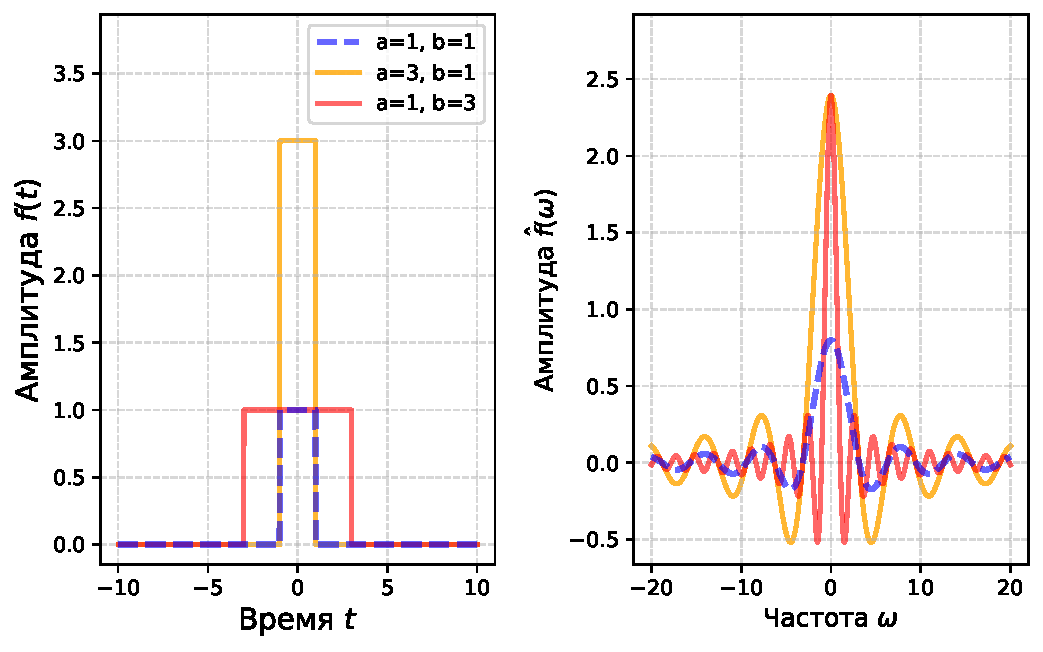
\includegraphics[width=1\linewidth]{imgs/1_rectangle.pdf}
    \caption{Временной оригинал и частотный спектр прямоугольного импульса}
\end{figure}

\    % Оставляем отступ
Прямоугольный импульс является классическим примером сигнала с жесткой пространственной локализацией и мгновенными разрывами первого рода на границах $|t| = b$. На графиках отчетливо проявляется следствие свойства линейности: увеличение амплитуды оригинала в 3 раза (оранжевый график) пропорционально растягивает спектр по вертикали, сохраняя точки пересечения оси частот. 

Взаимосвязь параметров ширины наглядно иллюстрирует свойство масштабирования: расширение импульса в пространстве (красный график, $b=3$) приводит к сильному сжатию его главного лепестка в частотной области и увеличению частоты осцилляций боковых лепестков. Медленное затухание амплитуды спектра (пропорционально $1/\omega$) напрямую обусловлено формой сигнала, получается так, что резкие перепады уровней в оригинале порождают бесконечный спектр высоких частот.

\newpage

\textbf{Треугольная функция}

Временной оригинал и частотный образ функции описываются выражениями:
\begin{equation*}
f(t) = \begin{cases} 
a - \frac{a}{b}|t|, & |t| \le b, \\ 
0, & |t| > b. 
\end{cases}
\quad \Longleftrightarrow \quad
\hat{f}(\omega) = \frac{1}{\sqrt{2\pi}}\frac{4a \sin^2\left(\frac{\omega b}{2}\right)}{b\omega^2}
\end{equation*}

\begin{figure}[H]
    \centering
    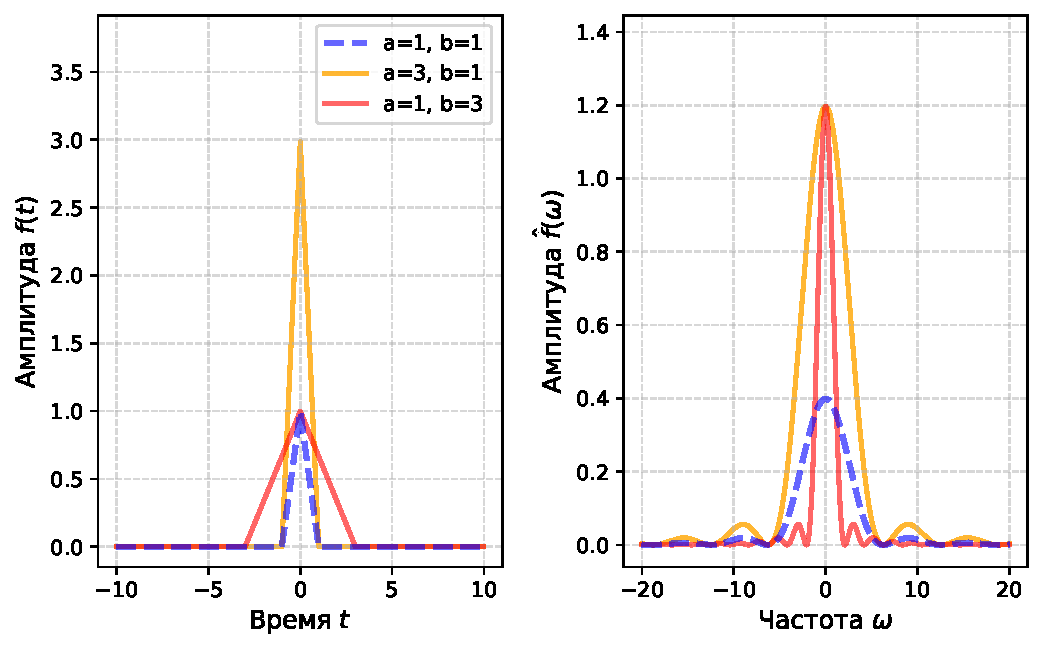
\includegraphics[width=1\linewidth]{imgs/2_triangle.pdf}
    \caption{Временной оригинал и частотный спектр треугольного импульса}
\end{figure}

\    
Треугольный импульс можно интерпретировать как результат свертки двух прямоугольных сигналов. 
С точки зрения математического анализа, такой сигнал является более гладким: 
если у прямоугольного импульса разрыв функции происходит в ней самой, 
то у треугольного импульса функция непрерывна, а разрыв наблюдается только у её первой производной.

Это свойство кардинально меняет поведение Фурье-образа. Спектр треугольной функции затухает 
значительно быстрее - обратно пропорционально квадрату частоты. 
Боковые лепестки спектра практически прижаты к нулю, 
а сам образ является строго неотрицательным из-за квадрата синуса в числителе. 
Геометрические зависимости сохраняются: увеличение параметра $b$ (красный график) 
локализует основную энергию сигнала в узком низкочастотном диапазоне.

\newpage

\textbf{Кардинальный синус}

Временной оригинал и частотный образ функции описываются выражениями:
\begin{equation*}
f(t) = a \text{sinc}(bt)
\quad \Longleftrightarrow \quad
\hat{f}(\omega) = \begin{cases} 
\frac{a}{b}\sqrt{\frac{\pi}{2}}, & |\omega| \le b \\ 
0, & |\omega| > b 
\end{cases}
\end{equation*}

\begin{figure}[H]
    \centering
    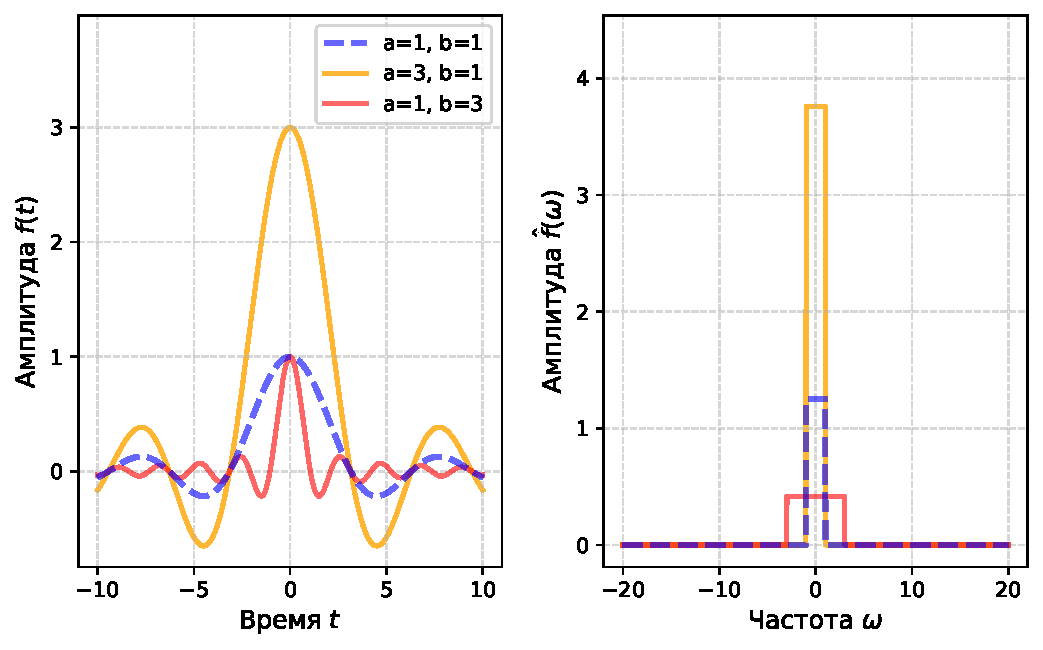
\includegraphics[width=1\linewidth]{imgs/3_sinc.pdf}
    \caption{Временной оригинал и частотный спектр кардинального синуса}
\end{figure}

\    
Исследование функции кардинального синуса демонстрирует свойство двойственности преобразования Фурье. 
Мы наблюдаем ситуацию, обратную прямоугольному импульсу: бесконечный во времени, плавно затухающий 
осциллирующий сигнал порождает идеально ограниченный частотный спектр. 

В радиотехнике и цифровой обработке сигналов такой образ соответствует идеальному фильтру нижних частот. 
Параметр $b$ здесь определяет полосу пропускания фильтра: чем больше $b$ (красный график), 
тем шире диапазон частот, которые пропускает система, и тем более сжатым и плотным становится импульс 
во временной области. И наоборот, низкочастотный кардинальный синус (синий график) 
сильно растянут во времени.

\newpage

\textbf{Функция Гаусса}

Временной оригинал и частотный образ функции описываются выражениями:
\begin{equation*}
f(t) = ae^{-bt^2}
\quad \Longleftrightarrow \quad
\hat{f}(\omega) = \frac{a}{\sqrt{2b}}e^{-\frac{\omega^2}{4b}}
\end{equation*}

\begin{figure}[H]
    \centering
    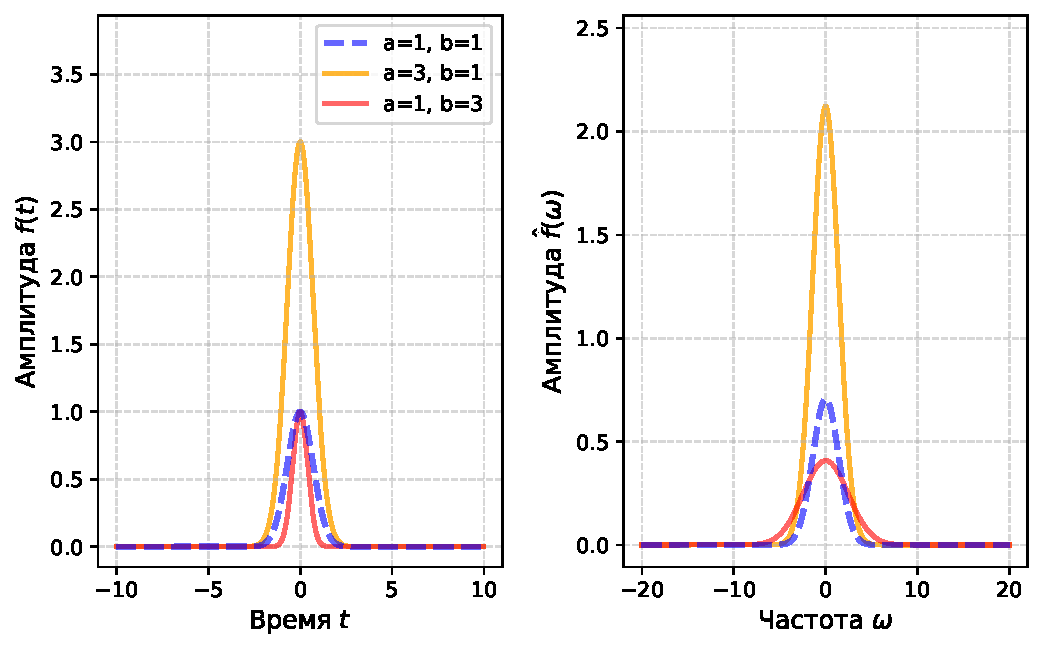
\includegraphics[width=1\linewidth]{imgs/4_gauss.pdf}
    \caption{Временной оригинал и частотный спектр функции Гаусса}
\end{figure}

\    
Функция Гаусса обладает уникальным математическим свойством - она инвариантна по форме относительно преобразования Фурье. Это означает, что частотный образ гауссоида качественно повторяет 
форму оригинала, оставаясь колоколообразной кривой без осцилляций и боковых лепестков. 

Отсутствие боковых лепестков объясняется абсолютной гладкостью функции Гаусса 
(она бесконечно дифференцируема). На данном семействе графиков идеально прослеживается 
соотношение неопределенностей: сужение колокола во временной области 
(синий и оранжевый графики имеют одинаковую ширину, но оранжевый выше) компенсируется в частотной 
области. Если же мы берем малое значение параметра затухания $b$ (красный график), то пологий во 
времени сигнал превращается в узкий высокоамплитудный пик на нулевой частоте.

\newpage

\textbf{Двустороннее затухание}

Временной оригинал и частотный образ функции описываются выражениями:
\begin{equation*}
f(t) = ae^{-b|t|}
\quad \Longleftrightarrow \quad
\hat{f}(\omega) = a \sqrt{\frac{2}{\pi}} \frac{b}{b^2 + \omega^2}
\end{equation*}

\begin{figure}[H]
    \centering
    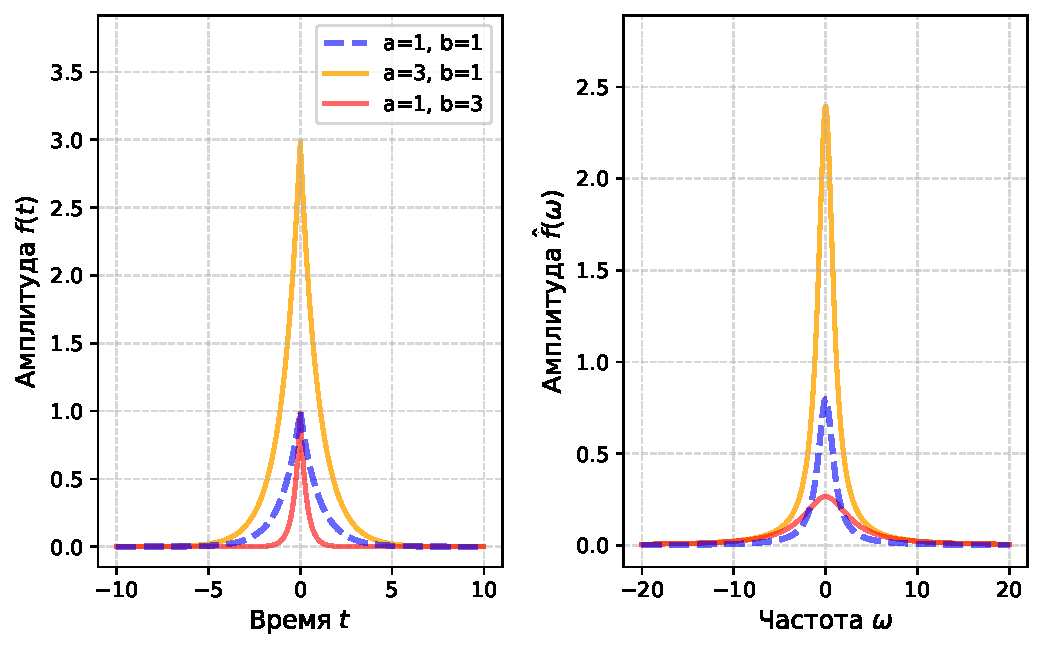
\includegraphics[width=1\linewidth]{imgs/5_exp.pdf}
    \caption{Временной оригинал и частотный спектр двустороннего экспоненциального затухания}
\end{figure}

\    
Экспоненциальное затухание представляет собой непрерывную функцию, первая производная которой образует излом строго в начале координат при $t = 0$. Согласно свойствам преобразования 
Фурье, именно наличие этого излома определяет поведение спектра: на высоких частотах 
амплитуда убывает обратно пропорционально квадрату частоты ($1/\omega^2$). По скорости затухания 
спектра этот сигнал аналогичен треугольному импульсу, который также имеет разрывы только в первой 
производной.

Поскольку в оригинале отсутствуют резкие прямоугольные границы, частотный спектр лишен волновых 
осцилляций и представляет собой гладкую спадающую кривую. При увеличении коэффициента 
затухания $b$ (красный график) сигнал мгновенно затухает во времени, что заставляет его спектр 
расплываться по частотной оси, распределяя энергию по широкому диапазону.

\newpage

\subsection{Проверка равенства Парсеваля}
Равенство Парсеваля для унитарного преобразования имеет следующий вид:
\begin{equation*}
    \int\limits_{-\infty}^{\infty} |f(t)|^2 dt = \int\limits_{-\infty}^{\infty}|\hat{f}(\omega)|^2d\omega
\end{equation*}

Для численной проверки данного равенства воспользуемся библиотекой \texttt{scipy} языка 
Python. Интегрирование оригиналов с конечным носителем проводилось строго в их 
аналитических границах, а образов - на бесконечном интервале с повышенными 
требованиями к точности интегрирования.

\textbf{Прямоугольная функция}\\
\begin{center}
\begin{tabular}{|c|c|c|c|}
    \hline
     $(a, b)$& $\int\limits_{-\infty}^{\infty} |f(t)|^2 dt$ & $\int\limits_{-\infty}^{\infty}|\hat{f}(\omega)|^2d\omega$ & Статус\\
     \hline
      (1, 1)& 2.000000 & 2.000000 & Выполняется \\
      \hline
      (3, 1)& 18.000000 & 17.999997 & Выполняется \\
      \hline
      (1, 3)& 6.000000 & 6.000006 & Выполняется\\
      \hline
\end{tabular}
\end{center}

\textbf{Треугольная функция}\\
\begin{center}
\begin{tabular}{|c|c|c|c|}
    \hline
     $(a, b)$& $\int\limits_{-\infty}^{\infty} |f(t)|^2 dt$ & $\int\limits_{-\infty}^{\infty}|\hat{f}(\omega)|^2d\omega$ & Статус\\
     \hline
      (1, 1)& 0.666667 & 0.666667 & Выполняется \\
      \hline
      (3, 1)& 6.000000 & 6.000000 & Выполняется \\
      \hline
      (1, 3)& 2.000000 & 2.000000 & Выполняется\\
      \hline
\end{tabular}
\end{center}

\textbf{Кардинальный синус}\\
\begin{center}
\begin{tabular}{|c|c|c|c|}
    \hline
     $(a, b)$& $\int\limits_{-\infty}^{\infty} |f(t)|^2 dt$ & $\int\limits_{-\infty}^{\infty}|\hat{f}(\omega)|^2d\omega$ & Статус\\
     \hline
      (1, 1)& 3.141592 & 3.141593 & Выполняется \\
      \hline
      (3, 1)& 28.274329 & 28.274334 & Выполняется \\
      \hline
      (1, 3)& 1.047199 & 1.047198 & Выполняется\\
      \hline
\end{tabular}
\end{center}

\textbf{Функция Гаусса}\\
\begin{center}
\begin{tabular}{|c|c|c|c|}
    \hline
    $(a, b)$& $\int\limits_{-\infty}^{\infty} |f(t)|^2 dt$ & $\int\limits_{-\infty}^{\infty}|\hat{f}(\omega)|^2d\omega$ & Статус\\
    \hline
    (1, 1)& 1.253314 & 1.253314 & Выполняется \\
      \hline
      (3, 1)& 11.279827 & 11.279827 & Выполняется \\
      \hline
      (1, 3)& 0.723601 & 0.723601 & Выполняется\\
      \hline
\end{tabular}
\end{center}

\newpage

\textbf{Двустороннее затухание}\\
\begin{center}
\begin{tabular}{|c|c|c|c|}
    \hline
     $(a, b)$& $\int\limits_{-\infty}^{\infty} |f(t)|^2 dt$ & $\int\limits_{-\infty}^{\infty}|\hat{f}(\omega)|^2d\omega$ & Статус\\
     \hline
     (1, 1)& 1.000000 & 1.000000 & Выполняется \\
      \hline
      (3, 1)& 9.000000 & 9.000000 & Выполняется \\
      \hline
      (1, 3)& 0.333333 & 0.333333 & Выполняется\\
      \hline
\end{tabular}
\end{center}

\textbf{Анализ результатов интегрирования:}\\
Полученные численные данные наглядно подтверждают выполнение теоремы Парсеваля. При этом наблюдается характерная закономерность, зависящая от спектральных свойств самих функций. Для абсолютно гладкой функции Гаусса, а также для непрерывных функций с быстрой сходимостью интегралов (треугольный импульс и двустороннее затухание со спадом спектра $1/\omega^2$) алгоритмы квадратурного интегрирования обеспечивают идеальное совпадение энергий до шестого знака после запятой.

Расхождения порядка $10^{-6}$, возникающие в случае прямоугольного импульса и 
кардинального синуса, имеют строгую математическую природу. Спектр прямоугольного импульса 
(функция \text{sinc}) и оригинал кардинального синуса обладают медленным затуханием порядка 
$1/\omega$ и бесконечным числом осцилляций на числовой оси. Численное суммирование площади таких 
медленно сходящихся колебаний на интервале $(-\infty, \infty)$ является сложной вычислительной 
задачей, и появление погрешности в последних разрядах обусловлено ограничением числа итераций 
алгоритма, а не нарушением физического закона сохранения энергии.

\newpage

\section{Комплексное преобразование}

Для выполнения данного задания выберем функцию двустороннего затухания $f(t) = ae^{-b|t|}$. Набор базовых параметров зафиксируем как $a=1$, $b=3$.\\

Рассмотрим функцию $g(t) = f(t + c)$, которая представляет собой исходный сигнал, сдвинутый во времени, и имеет вид $g(t) = ae^{-b|t+c|}$.\\

Выполним унитарное преобразование Фурье. Согласно свойству сдвига, временной сдвиг сигнала на величину 
$c$ эквивалентен умножению его спектра на комплексную экспоненту $e^{i\omega c}$:

\begin{equation*}
    \begin{split}
    \hat{g}(\omega) &= \frac{1}{\sqrt{2\pi}} \int_{-\infty}^{\infty} a e^{-b|t+c|} e^{-i\omega t} dt = \frac{a e^{i\omega c}}{\sqrt{2\pi}} \left( \int_{-\infty}^{0} e^{(b-i\omega)t} dt + \int_{0}^{\infty} e^{-(b+i\omega)t} dt \right) =\\
    & = \frac{a e^{i\omega c}}{\sqrt{2\pi}} \left( \frac{1}{b-i\omega} + \frac{1}{b+i\omega} \right) = a \sqrt{\frac{2}{\pi}} \frac{b}{b^2 + \omega^2} e^{i\omega c}
    \end{split}
\end{equation*}

Таким образом, мы получили:\\
\textbf{Оригинал:} $g(t) = ae^{-b|t+c|}$\\
\textbf{Образ:} $\hat{g}(\omega) = a \sqrt{\frac{2}{\pi}} \frac{b}{b^2 + \omega^2} e^{i\omega c}$\\

Для наглядной визуализации влияния параметра $c$ на сигнал и его спектр, 
зададимся следующим набором значений:
\begin{center}
    \begin{tabular}{|c|c|c|c|}
        \hline
        $c_1$ & $c_2$ & $c_3$ & $c_4$ \\
        \hline
         -3.0 & -0.5 & 1.0 & 2.0 \\
         \hline
         Синий & Оранжевый & Зелёный & Красный \\
         \hline
    \end{tabular}
\end{center}

Построим графики $g(t)$ с заданными параметрами:
\begin{figure}[H]
    \centering
    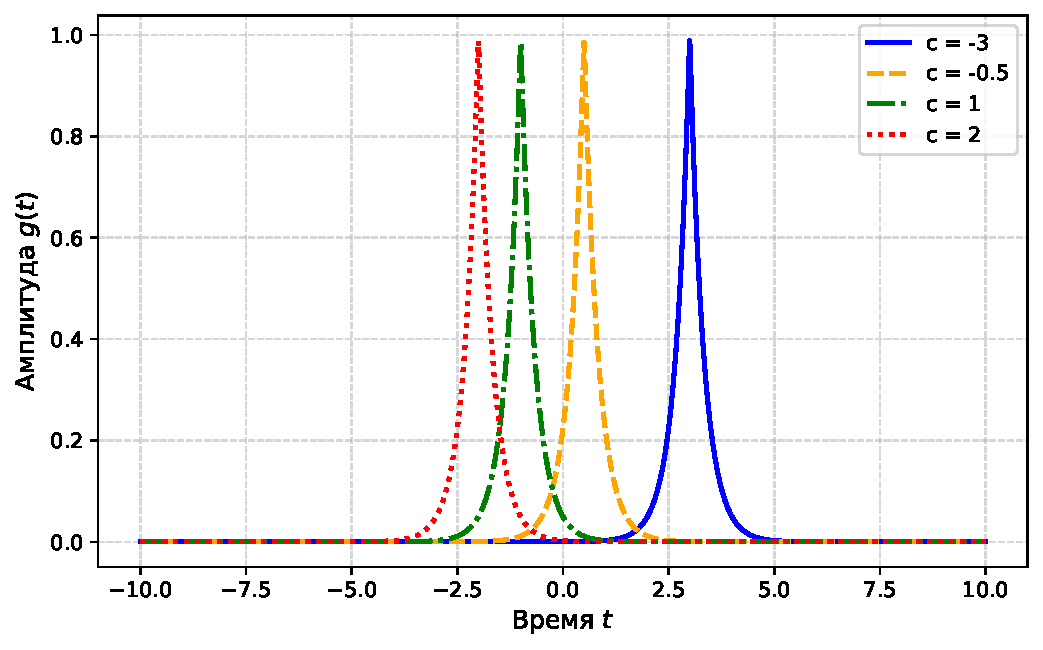
\includegraphics[width=1\linewidth]{imgs/task2_originals.pdf}
    \caption{Оригиналы сдвинутых функций $g(t)$}
\end{figure}

По графикам видно, что математический сдвиг аргумента на $+c$ приводит к смещению 
графика функции в сторону отрицательных значений $t$, а сдвиг на $-c$ - 
в сторону положительных значений времени.\\

Для анализа поведения Фурье-образа воспользуемся формулой Эйлера: 
\begin{equation*}
    e^{i\omega c} = \cos(\omega c) + i \sin(\omega c)
\end{equation*} 
Разложим комплексный спектр на вещественную и мнимую составляющие, а также найдем его абсолютное значение:

\begin{equation*}
    \begin{split}
    Re(\hat{g}(\omega)) &= a \sqrt{\frac{2}{\pi}} \frac{b}{b^2 + \omega^2} \cos(\omega c)\\
    Im(\hat{g}(\omega)) &= a \sqrt{\frac{2}{\pi}} \frac{b}{b^2 + \omega^2} \sin(\omega c)\\
    |\hat{g}(\omega)| &= a \sqrt{\frac{2}{\pi}} \frac{b}{b^2 + \omega^2}
    \end{split}
\end{equation*}

Построим соответствующие графики частотных образов:
\begin{figure}[H]
    \centering
    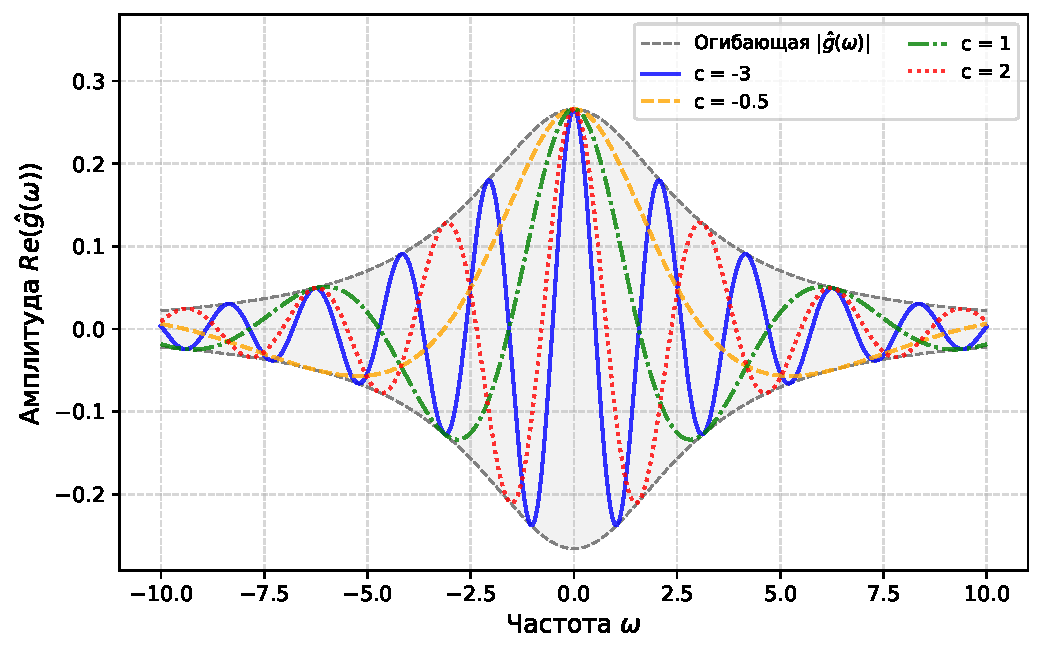
\includegraphics[width=1\linewidth]{imgs/task2_re.pdf}
    \caption{Спектр: Вещественная часть $Re(\hat{g}(\omega))$}
\end{figure}

\begin{figure}[H]
    \centering
    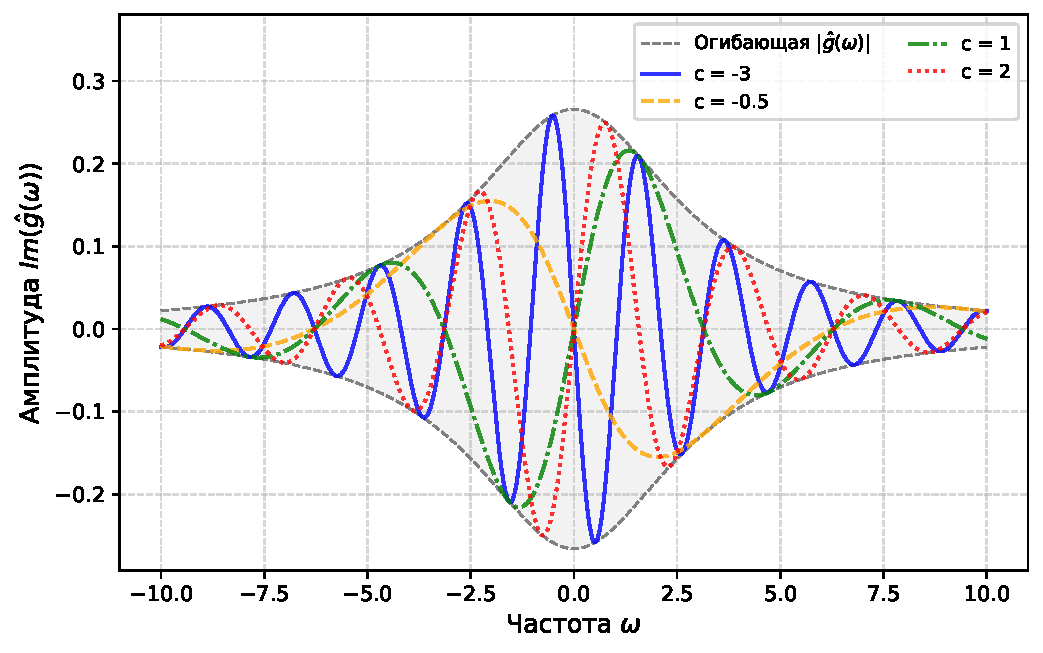
\includegraphics[width=1\linewidth]{imgs/task2_im.pdf}
    \caption{Спектр: Мнимая часть $Im(\hat{g}(\omega))$}
\end{figure}

\begin{figure}[H]
    \centering
    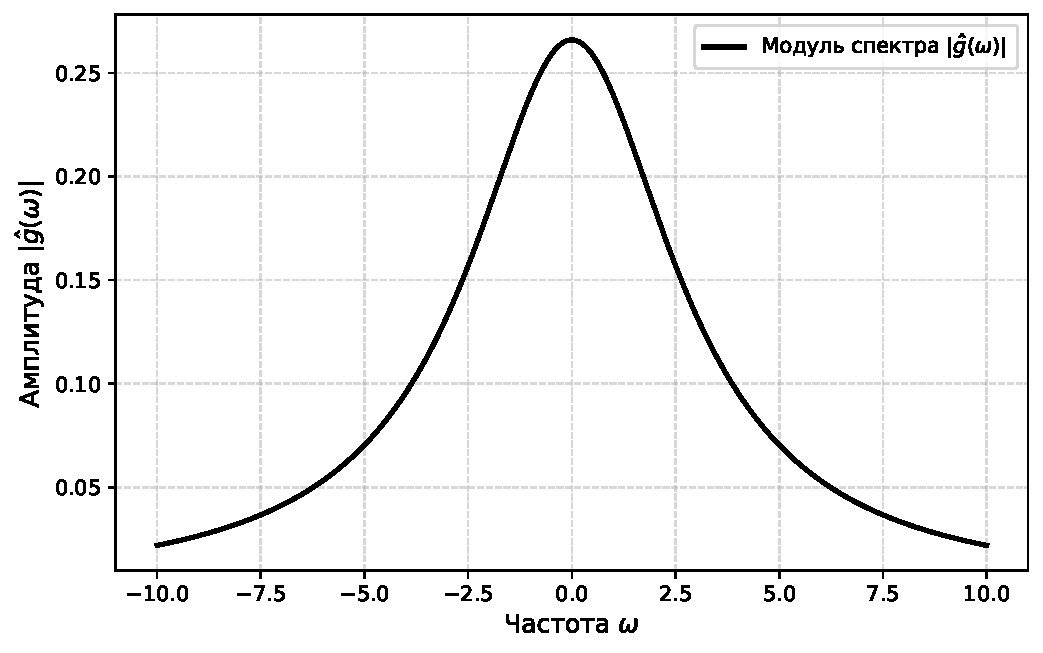
\includegraphics[width=1\linewidth]{imgs/task2_mod.pdf}
    \caption{Спектр: Абсолютное значение $|\hat{g}(\omega)|$}
\end{figure}

\textbf{Выводы по результатам моделирования:}\\
Анализ графиков подтверждает фундаментальное свойство преобразования Фурье: 
временная задержка сигнала не изменяет энергетический спектр 
сигнала - график модуля $|\hat{g}(\omega)|$ остается неизменным и выступает в 
роли амплитудной огибающей. 

Однако сдвиг вносит линейный набег фазы, который проявляется в виде гармонических осцилляций 
вещественной и мнимой частей спектра. Чем больше абсолютное значение временного 
сдвига $|c|$, тем выше частота этих осцилляций под огибающей. Знак параметра $c$ определяет 
направление начальной фазы синусоиды в мнимой части спектра.

\newpage

\section{Музыкальное задание}

Для выполнения данного задания был выбран аудиофрагмент "Аккорд 28". 
С помощью библиотеки \texttt{librosa} на языке Python был произведен импорт звуковых данных. 
В результате извлечения мы получили дискретный массив амплитуд сигнала во времени, на 
основе которого построен временной график звучания аккорда.

\begin{figure}[H]
    \centering
    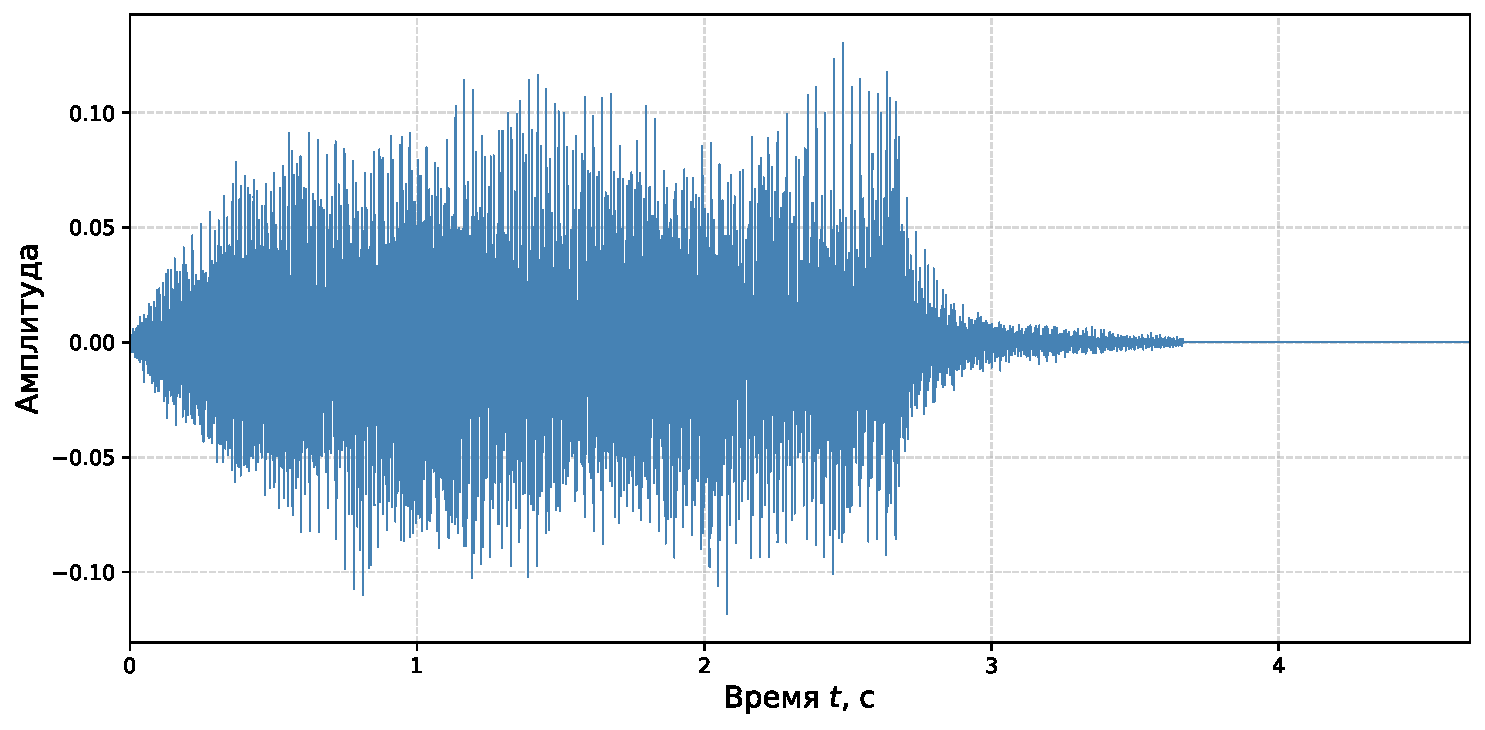
\includegraphics[width=1\linewidth]{imgs/mus_graph.pdf}
    \caption{Осциллограмма аккорда 28}
    \label{fig:task3}
\end{figure}

Для перехода в частотную область и получения Фурье-образа мы применили численное 
интегрирование. Вычисление интеграла производилось методом трапеций с помощью 
векторизованной функции \texttt{trapezoid} из библиотеки \texttt{scipy.integrate}. 
По результатам интегрирования был получен массив амплитуд спектра, на котором 
с помощью функции \texttt{find\_peaks} выделены пиковые значения, 
соответствующие доминирующим гармоникам.

\begin{figure}[H]
    \centering
    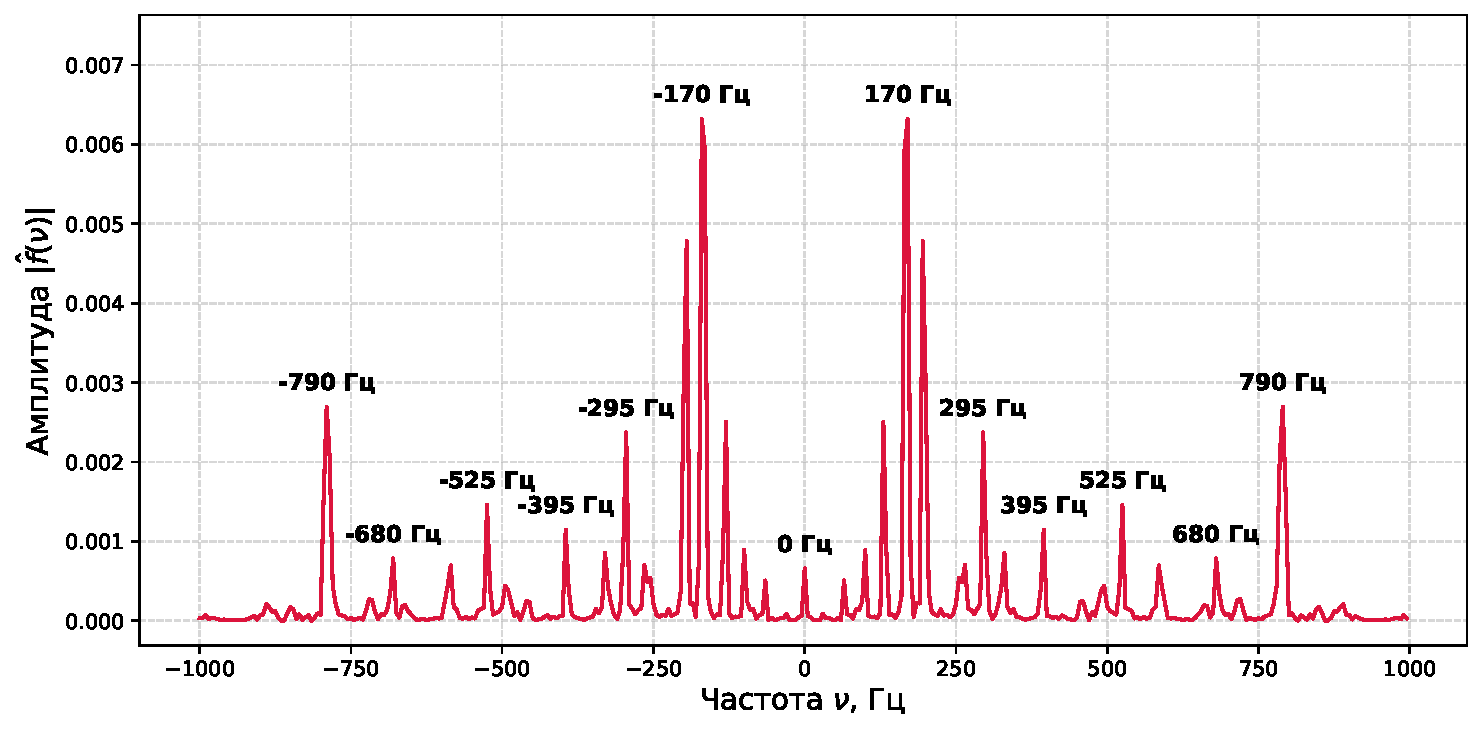
\includegraphics[width=1\linewidth]{imgs/furie_music.pdf}
    \caption{Фурье-образ аккорда 28}
    \label{fig:task3_fourier}
\end{figure}

Амплитуда на конкретной частоте отражает энергетический вклад соответствующей ноты в общее звучание аккорда. На спектрограмме отчетливо зафиксированы 6 ярко выраженных пиков: 170 Гц, 295 Гц, 395 Гц, 525 Гц, 680 Гц и 790 Гц.

Однако сам аккорд состоит всего из четырех базовых нот. 
Наличие дополнительных частот (680 Гц и 790 Гц) объясняется акустической 
природой реальных музыкальных инструментов - явлением обертонов. 
Звучание любого сложного музыкального инструмента, будь то физические колебания струны, 
работа акустического резонатора или сигнал электронного осциллятора содержит не только несущую частоту, 
но и кратные ей высокочастотные колебания, которые формируют уникальный тембр инструмента. 

В исследуемом спектре пик на 680 Гц является третьим обертоном 
базовой частоты 170 Гц, 
а пик на 790 Гц - первым обертоном частоты 395 Гц. 

При сопоставлении полученных частот с эталонными значениями равномерно 
темперированного строя наблюдается незначительное расхождение. 
Данная погрешность носит алгоритмический характер и обусловлена выбранной разрешающей 
способностью частотной сетки при численном интегрировании, мы выбрали шаг дискретизации $\Delta\nu = 5$ Гц. Кроме того, отклонения частот являются 
нормой для реальных и синтезированных тембров из-за эффектов акустической негармоничности 
и детюна, придающих звуку объем. Тем не менее, точности алгоритма оказалось 
более чем достаточно для однозначной идентификации нотного состава аккорда.

\begin{center}
\begin{tabular}{|c|c|c|}
    \hline
    \textbf{Частота (Гц)} & \textbf{Западная нотация} & \textbf{Русская нотация} \\
    \hline
    170 & F3 & Фа малой октавы \\
    \hline
    295 & D4 & Ре первой октавы \\
    \hline
    395 & G4 & Соль первой октавы \\
    \hline
    525 & C5 & До второй октавы \\
    \hline
\end{tabular}
\end{center}

\newpage

\section{Выводы}

В ходе выполнения лабораторной работы было проведено исследование 
непрерывного преобразования Фурье, охватывающее как аналитические методы расчета, 
так и численное моделирование сигналов. Математический аппарат интеграла Фурье позволил 
нам перейти от анализа периодических рядов к работе с одиночными импульсами непериодической 
природы путем предельного перехода периода к бесконечности.

В рамках первой части работы были получены аналитические выражения частотных 
образов для пяти типовых сигналов. Построенные графики наглядно подтвердили 
фундаментальные свойства преобразования: теоремы подобия, линейности и 
двойственности, а также продемонстрировали прямую зависимость между гладкостью 
функции и скоростью убывания её амплитудного спектра. Выполнение закона сохранения 
энергии при переходе из временной в частотную область было подтверждено 
путем численной проверки равенства Парсеваля.

Далее, исследование комплексного преобразования на примере функции двустороннего 
затухания доказало математическую справедливость теоремы о запаздывании. 
Было установлено, что временной сдвиг сигнала оставляет модуль образа абсолютно инвариантным, 
однако вносит линейный фазовый набег. Этот набег физически проявляется в виде 
высокочастотных гармонических осцилляций вещественной и мнимой частей комплексного спектра.

Наконец, при решении прикладной задачи был написан алгоритм 
численного интегрирования для реального аудиофрагмента. Переход из временной области 
в частотную позволил разложить сложный акустический сигнал на 
элементарные гармонические составляющие. Алгоритмический поиск пиковых амплитуд 
дал возможность не только идентифицировать базовые частоты, соответствующие конкретным 
нотам музыкального аккорда, но и выявить обертоны, формирующие тембр звучания.

Таким образом, преобразование Фурье доказало свою высочайшую эффективность как 
фундаментальный инструмент цифровой обработки сигналов, позволяющий извлекать 
скрытые частотные характеристики из сложных временных рядов.

\newpage

\section{Приложение}

\lstinputlisting[language=Python, caption={Построение графиков из 1 задания}]{code/task_1_graphs.py}

\lstinputlisting[language=Python, caption={Проверка равенства Парсеваля}]{code/Parseval_task_1.py}

\lstinputlisting[language=Python, caption={Построение графиков из 2 задания}]{code/2task_all.py}

\lstinputlisting[language=Python, caption={Численное вычисление преобразования Фурье и выделение гармоник звукового сигнала}]{code/music.py}

\end{document}